%*******************************************************************************
%****************************** Fourth Chapter *********************************
%*******************************************************************************

\chapter{Characterisation of III-Nitride Microdisk Cavities}
\label{Microdisk Chapter}
\ifpdf
    \graphicspath{{Chapter2/Figs/Raster/}{Chapter2/Figs/PDF/}{Chapter2/Figs/}}
\else
    \graphicspath{{Chapter2/Figs/Vector/}{Chapter2/Figs/}}
\fi


\section[Background]{Background}

Microcavities possess particular optical properties, as discussed in section \ref{cavity section}. Strongly-coupled cavities are crucial in accomplishing important quantum information processing tasks such as controlled coherent coupling and the entanglement of quantum systems \cite{Hennessy2007}. Weakly-coupled microcavity systems have many applications in optoelectronic devices such as high efficiency, low threshold lasers \cite{Vahala2003}. Applications for both strong and weak coupling cavities are discussed in more detail in section \ref{cavity section}.
\\ Though various geometries for cavities exist, in this chapter we will specifically address III-nitride microdisk cavities. Microdisk III-nitride cavities have presented several challenges in terms of fabrication due to the chemical and thermal properties of GaN discussed in section \ref{microdisk section}. Currently, one of the most effective method for the fabrication of III-nitride microdisk cavities is PEC etching of an InGaN sacrificial superlattice \nomenclature[z-SSL]{SSL}{Sacrificial Superlattice} (SSL) \cite{Puchtler2015}. This in itself presents issues, as El-Ella \textit{et al.} have shown that the growth of the InGaN SSL with a quantum dot (QD) layer can introduce dislocations into the structure \cite{El-Ella2011a}. Furthermore, PEC etching can be a difficult process to control as it is heavily dependent on conductivity and hence can be defect-selective \cite{Visconti2001,Youtsey1999,Youtsey1998} and dopant-selective \cite{Youtsey1999}, occasionally resulting in protrusions or roughness \cite{Puchtler2015} on the etched underside of microdisk cavities which can heavily influence microdisk Q-factor \cite{Puchtler2015}. The work contained in this chapter is a microscopy-based investigation into the structural properties of GaN/InGaN microdisk cavities.

\subsection{PEC etching}
\label{microdisk fab section}
As discussed in section \ref{microdisk section}, the ability to perform an effective 'undercut' is a crucial aspect in the fabrication of III-nitride microcavities. PEC etching is a commonly used technique to achieve an undercut microdisk and will be introduced here.
PEC etching was first reported in III-nitrides by Minsky \textit{et al.} \cite{Minsky1996}, and is an extremely effective method to perform selective etching as it can be defect-selective and bandgap-selective. To achieve an undercut on a III-nitride microdisk the following set-up is typically used: a GaN filter is used to absorb light emitted by a Xenon lamp, allowing light of wavelength longer than ~360nm to interact with the structure thus ensuring the majority of carriers are generated in the sacrificial InGaN layer. Holes generated by the incident light diffuse toward the surface of the InGaN layer which in this case acts as an anode whilst the electrons diffuse toward to the metal cathode due to both the overall potential in the connected cell and the band-bending occurring at the surfaces. This process is shown schematically in Fig.\ref{PECetch}.

\begin{figure}[h]
	\centering
	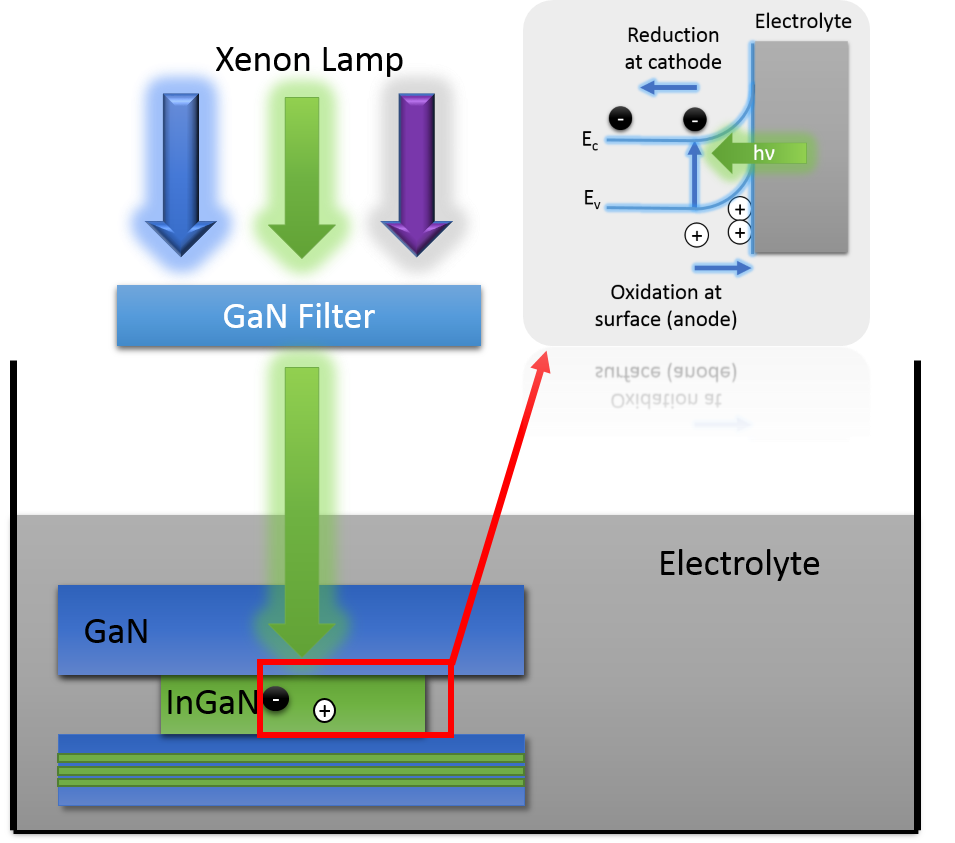
\includegraphics[width=0.8\textwidth]{Figs/Ch4/PEC.png}
	\caption {PEC etching set-up, with the charge transfer process shown in the inset.}
	\label{PECetch}
\end{figure}
\FloatBarrier 

The excess concentration of holes at the sacrificial layer surface drives the oxidation of InGaN, forming $\mathrm{Ga_{2}O_{3}, In_{2}O_{3}}$ and $\mathrm{N_{2}}$, while at the cathode a reduction process is driven by the excess electrons. The oxide generated by the reduction process is then dissolved in the electrolyte, thus etching the sacrificial layer. It is clear that the etch rate of the sacrificial layer is governed by several factors: the rate of generation of the photo-generated electron hole pairs, their diffusion rates towards the anode or cathode, and the concentration of the electrolyte (HCl in this case). It is due to this photo-generated carrier concentration dependence that the PEC etching process is defect and dopant selective.

\subsection{Whisker Generation in PEC Etching}
\label{Whisker section}
Youtsey \textit{et al.} demonstrated the ability of dislocations to hinder the progress of PEC etching and used this to determine the dislocation density of n-type GaN films. Unetched material (or ‘whiskers’) remained at dislocation sites after the PEC etching process due to the electrically active nature of dislocations in GaN, as shown in Fig. \ref{PECwhiskeryoutsey}.

\begin{figure}[h]
 	\centering
 	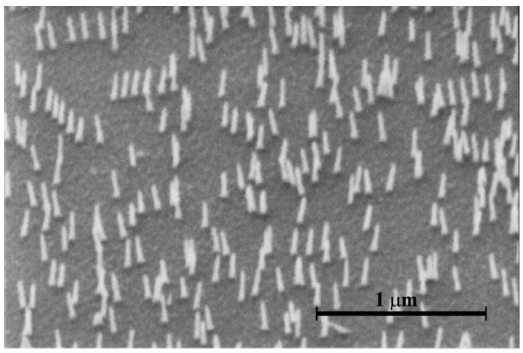
\includegraphics[width=0.8\textwidth]{Figs/Ch4/youtseywhisker.png}
 	\caption {SEM image of whiskers produced by etching of dislocations in an MOCVD GaN film grown on a silicon carbide (SiC) substrate. Reproduced from \cite{Youtsey1999}}
 	\label{PECwhiskeryoutsey}
\end{figure}
\FloatBarrier 

It was confirmed through cross-sectional TEM that both mixed and edge dislocations result in the formation of whiskers \cite{Youtsey1998}.\\
The mechanism through which the presence of dislocations impedes the PEC etching process relates to the charge trapping property of TDs: it has been suggested based on cathodoluminescence (CL) studies that TDs act as non-radiative recombination centres, as mentioned in section \ref{dislocation section}. In this case, photogenerated holes in the vicinity of TDs would be prevented from diffusing to the epilayer surface thus resulting in unetched material. There is also evidence for negatively charged TDs in n-type GaN \cite{Cherns2000}, which could lead to hole-trapping at TDs presenting an alternative or additional explanation for the reduction in surface hole concentration and thus reduced etch rate in areas adjacent to TDs \cite{Youtsey1998}.

\subsection{Q-factor Reduction in Microdisks}
\label{Q-factor reduction}
El-Ella \textit{et al.} first demonstrated the effect of dislocations on the Q-factor of GaN microdisks containing an InGaN QD active layer. By carefully controlling the In compostion of the SSL, the authors were able to produce two sets of microdisks, one with a dislocation density of $3 \times 10^{9} cm^{-2}$ (sample A) and the other with a lower density of $7 \times 10^{8} cm^{-2}$ (sample B). As expected, microdisks fabricated from sample A exhibited a larger density of whiskers on the underside of the disk. SEM was used to establish that 90$\%$ of disks fabricated from material A exhibited whiskers, compared to only 20$\%$  of disks fabricated from structure B. The difference between the two samples in terms of Q-factor is illustrated in Fig.\ref{El-Ellacomp} which includes data for eight microdisks fabricated from each sample. 

\begin{figure}[h]
	\centering
	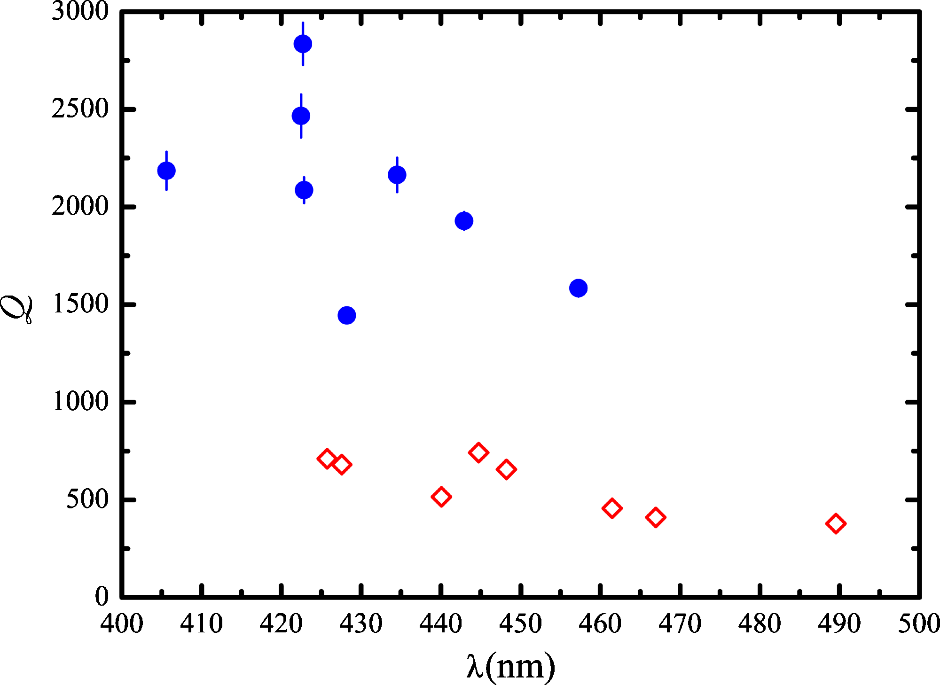
\includegraphics[width=0.8\textwidth]{Figs/Ch4/elellacomp.png}
	\caption {Q values from eight modes of microdisks fabricated from structure A(\textcolor{red}{$\lozenge$}) and B ((\textcolor{blue}{$\Bigcdot$}). Reproduced from \cite{El-Ella2011}.}
	\label{El-Ellacomp}
\end{figure}
\FloatBarrier 

All microdisks fabricated from sample B show a larger Q-factor than all microdisks from sample A. The average Q-factors for microdisks fabricated from samples A and B were 600 and 2000 respectively, suggesting a strong correlation between Q-factor and dislocation density \cite{El-Ella2011}.\\
Puchtler \textit{et al.} addressed these issues by identifying not only the number but also the position of TDs in individual microdisk cavities and evaluating the effect of these parameters on microdisk Q-factors\cite{Puchtler2015}.  Unlike the study by El-Ella \textit{et al.}, this work correlated the performance of each individual device structure with its specific structure. In this study, dark spots in CL images (arising from non-radiative recombination as discussed in section \ref{dislocation section}) were used as a signature for the presence of dislocations, and hence whiskers.\\
The authors established the correspondence of dark spots in the CL to whiskers by comparing plan-view panchromatic CL images with side-view SEM images of the microdisks. The results of these correlative measurements are shown in Fig.\ref{puchtlerdislocation}.

\begin{figure}[h]
	\centering
	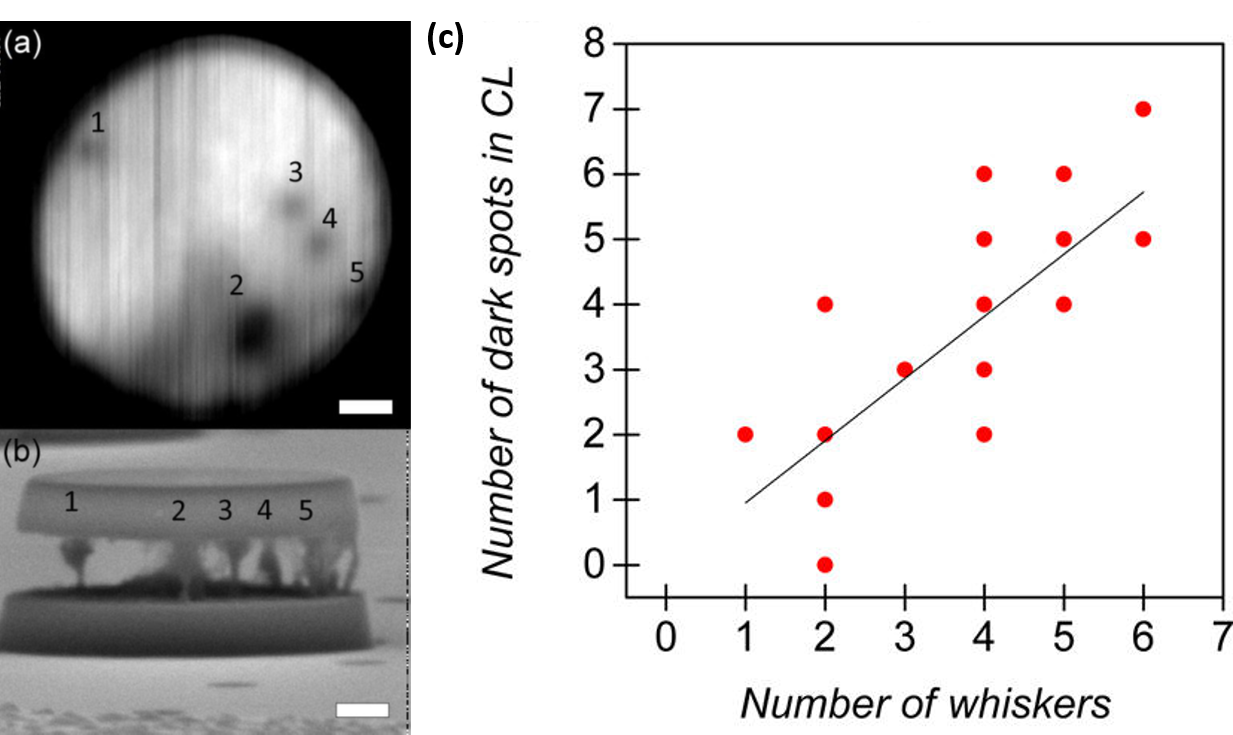
\includegraphics[width=1\textwidth]{Figs/Ch4/puchtlerdislocation.png}
	\caption {a) Sample plan-view CL b) Corresponding side-view SEM image of an undercut microdisk with whiskers corresponding to the dark spots shown in a). c) Relationship between whiskers on the underside and dark features counted in plan-view CL. Adapted from \cite{Puchtler2015}.}
	\label{puchtlerdislocation}
\end{figure}
\FloatBarrier 

Following this, the authors reported the correlation between dislocation number and position and Q-factor extracted from the modal peaks in micro-PL. Whilst dislocation number and microdisk Q-factor were shown to be inversely correlated, this was found to hold true only for dislocations located at a distance > 0.4 $\mu$m from the centre, suggesting only dislocations located within the outer-periphery of the microdisks (where the WGMs are confined as discussed in section \ref{microdisk section}) have an effect on Q-factor. These results are summarised in Fig.\ref{puchtlerdistance}.

\begin{figure}[h]
	\centering
	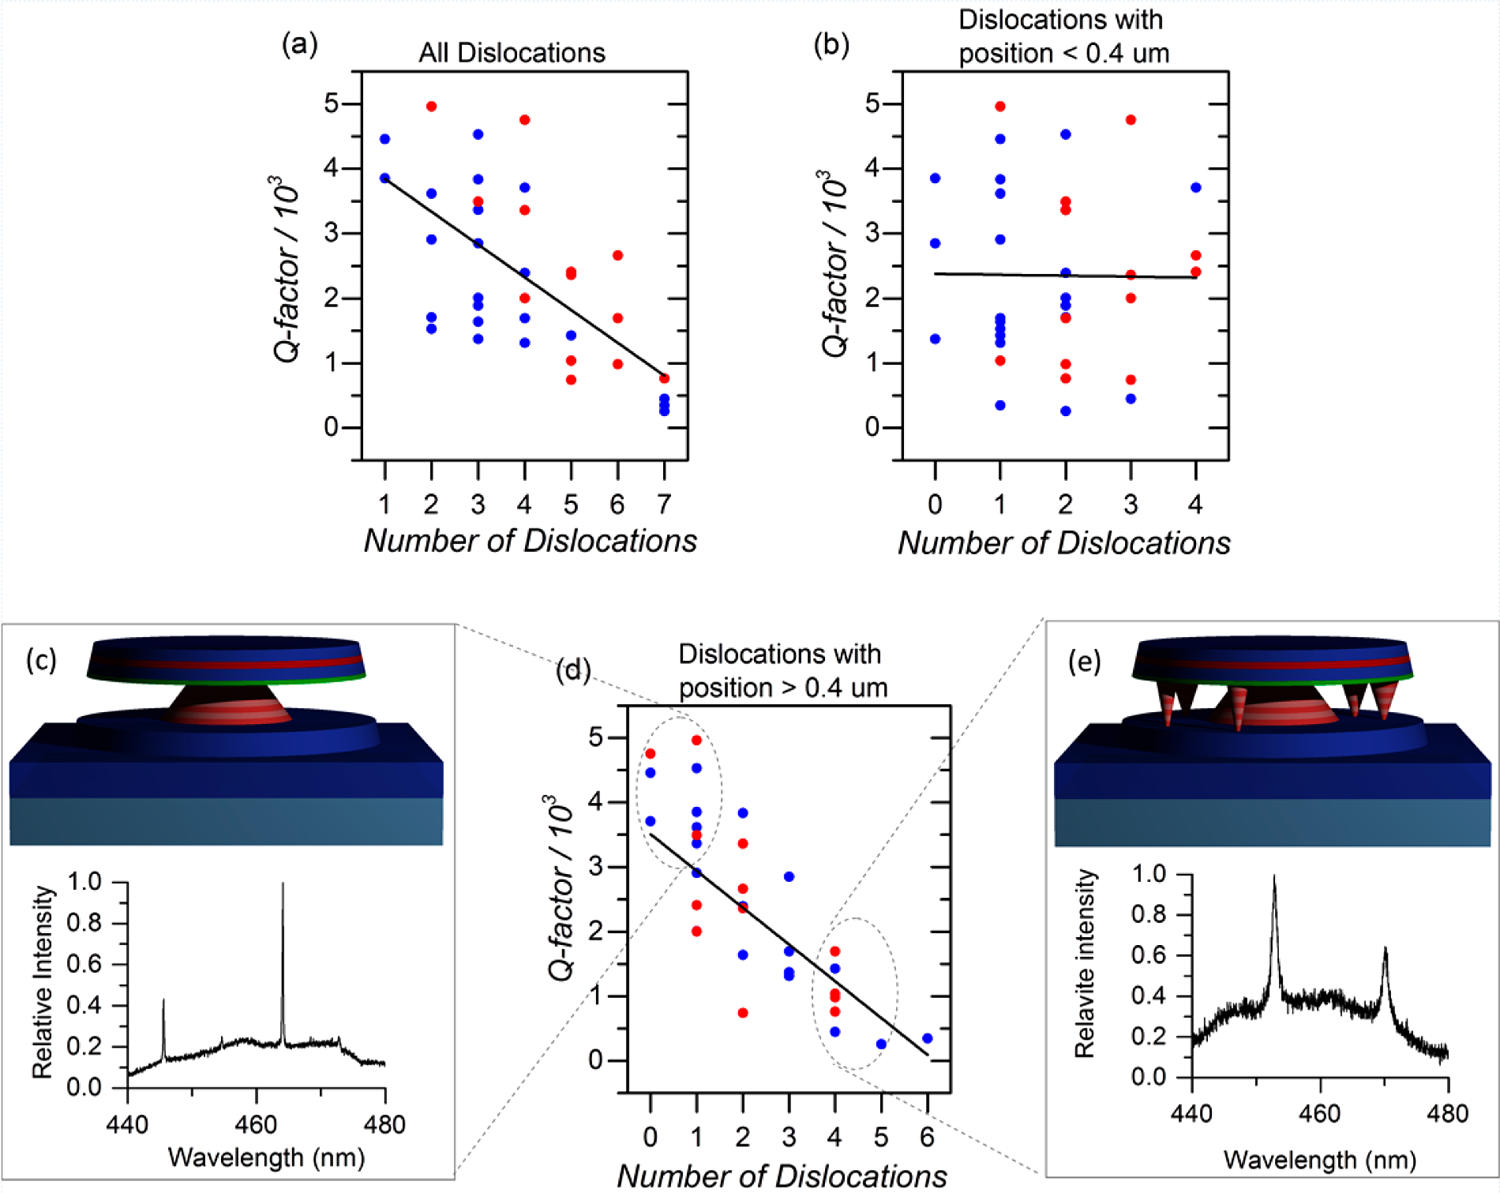
\includegraphics[width=1\textwidth]{Figs/Ch4/puchtlerdistance.png}
	\caption {a)Microdisk Q-factor vs. threading dislocation number for radial positions: a) 0- 0.6 $\mu$m b) < 0.4 $\mu$m d) >0.4 $\mu$m for QD (blue) and QW (red) containing microdisks. c) and e) show a schematic of, and representative PL spectrum taken from microdisks of low and high dislocation number in the periphery of the disks. Reproduced from \cite{Puchtler2015}.}
	\label{puchtlerdistance}
\end{figure}
\FloatBarrier 

The mechanism behind the deleterious effect of TDs on Q-factor were investigated by Puchtler \textit{et al.} through the use of finite difference time domain (FDTD) simulations \cite{Puchtler2015}. The presence of a whisker on the underside of a microdisk was simulated as a pyramidal protrusion with a range of dimensions and positions on the underside, producing results which suggest the Q-factor of the first order WGM decreases as the position of the whisker approaches the periphery of the microdisk and provides a radiative pathway for light confined in this region to escape \cite{Puchtler2015}. The results of these simulations are shown in Fig.\ref{puchtlersim}.
\begin{figure}[ht]
	\centering
	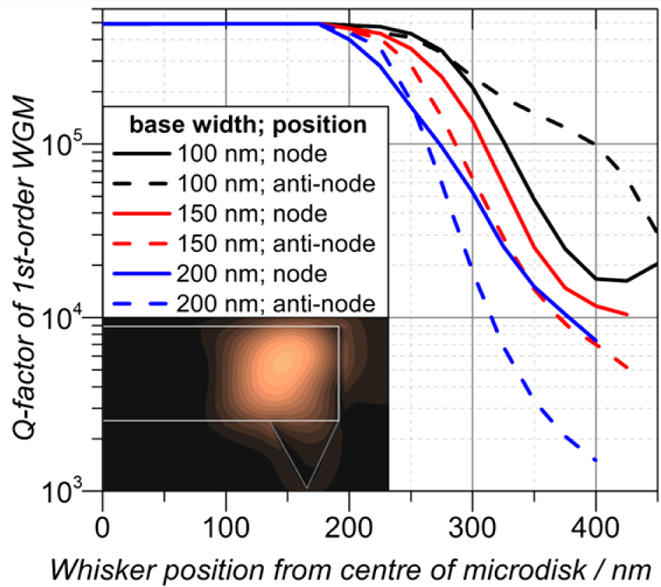
\includegraphics[width=0.7\textwidth]{Figs/Ch4/puchtlersim}
	\caption {Effect of radial position on the influence of a whisker on microdisk Q-factor. The whisker was simulated as a pyramid with a height of 150 nm and base widths of 100, 150, and 200 nm. The inset shows a side-on view of the field profile for a whisker located at the edge of the microdisk: light leaks into the whisker region and is radiated, thus introducing loss in the cavity. Reproduced from \cite{Puchtler2015}.}
	\label{puchtlersim}
\end{figure}
\FloatBarrier 

TDs have been shown to increase impurity levels at dislocation cores and in an extended region affected by their associated strain field during sample growth. TEM studies of dislocations have revealed strain related changes in doping occuring on the scale of several nanometres\cite{Rhode2013,Horton2015}. Threading dislocations can also have associated vacancy states giving rise to ‘yellow-band’ optical transitions, though these are far away from the wavelength range of III-nitride cavities \cite{Xin2000,Elsner1997}. In considering the impact of these factors  on absorption in the micodisk, Puchtler \textit{et al.} reported no significant effect on cavity Q-factor for linear attenuation coefficients up to $10^{9} cm^{-1}$ (several orders of magnitude greater than the expected value for highly doped GaN \cite{Ambacher1996}) associated with dislocations modelled as a cylinder of radius 4 nm.


\section[Experimental]{Microdisk Characterisation}
In this section we will report on the experimental microscopy work performed on microdisks. A FIB based lamella preparation method was developed in order to prepare TEM samples from the microdisks, allowing for the observation of a dislocation in a whisker from the underside of a microdisk as well as the characterisation of the microdisk active region. Furthermore, FIB tomography experiments were performed on the microdisk, allowing us to further characterise the structural properties of the microdisks.

\subsection{Samples}
\label{microdisk samples}
Samples for this study were grown on \textit{c}-plane GaN on a sapphire substrate. The active layers of the structure consist of three InGaN layers(QW or QD) in a 200 nm cavity membrane grown above a SSL $\mathrm{In_{x}Ga_{1-x}N/In_{y}Ga_{1-y}N}$ where x = 0.005 and y = 0.065. The purpose of the alternating In composition SSL is to confine carriers generated during the PEC process into localised regions. An unmodulated In composition would result in the separation of electron-hole pairs due to the inherent polarization fields present in InGaN, resulting in asymmetric etching \cite{El-Ella2011a}. The bottom of the microdisk membrane contains 20 nm $\mathrm{Al_{0.2}Ga_{0.8}}N$ layer which restricts the photo-generated carriers from the PEC process within the SSL, acting as an etch stop during undercutting and reducing damage to the microdisk membrane. The SSL is grown on a 500 nm \textit{n}-GaN layer which provides a highly conductive pathway for photo-generated carriers to be removed by propagating to an electrical contact. A schematic of the structure following the PEC undercut is shown in Fig.\ref{Puchtlerudiskimage}.

\begin{figure}[ht]
	\centering
	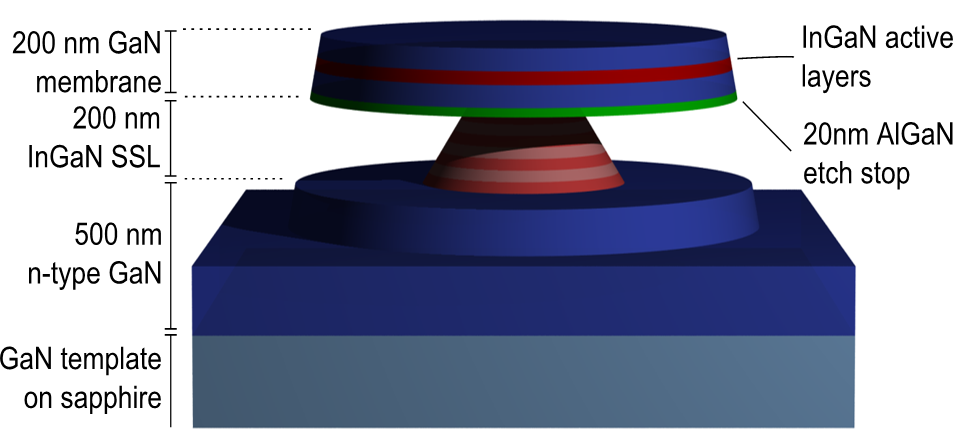
\includegraphics[width=0.7\textwidth]{Figs/Ch4/puchtlerimage}
	\caption {Schematic of the microdisk structure. Courtesy of Dr. T. Puchtler.}
	\label{Puchtlerudiskimage}
\end{figure}
\FloatBarrier 
	

\subsection{Whisker Analysis}

In sections \ref{Whisker section} we have discussed the manner in which dislocations hinder the PEC etching process and cause the formation of 'whiskers' on the underside of microdisk. Furthermore we have addressed the deleterious effect of these whiskers on microdisk Q-factor in section \ref{Q-factor reduction}. In this section we will present FIB/SEM techniques developed in order to produce TEM lamellae from delicate structures such as microdisks which have allowed for the direct observation of a TD in a whisker from a microdisk using TEM.

\subsection{FIB/SEM Sample Preparation}
\label{udiskFIBsection}
The microdisks studied here were found to be extremely sensitive to ion-beam damage during Pt deposition, even with a protective electron beam Pt layer deposited first. As such for the preparation of delicate structures it is key to restrict the usage of the ion-beam as much as possible. \\
In order to isolate a whisker on the underside of a microdisk for TEM examination, a target whisker is identified, and the sample is rotated in the FIB/SEM chamber to ensure optimal whisker orientation with respect to the TEM lamella, as shown in Fig.\ref{FIBwhisk}.

\begin{figure}[h]
	\centering
	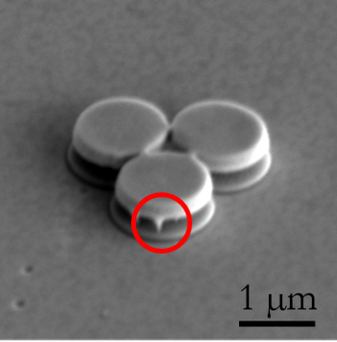
\includegraphics[width=0.5\textwidth]{Figs/Ch4/FIBwhisk}
	\caption {SEM micrograph taken at 3 kV and 0.16 nA of a PEC undercut microdisk with a whisker circled in red.}
	\label{FIBwhisk}
\end{figure}
\FloatBarrier 

A thick (approx. 2 $\mathrm{\mu m}$) protective layer of electron beam Pt is deposited on the surface of the microdisk. It is crucial to avoid using the ion-beam in this step to deposit Pt due to the fragility of the thin microdisk membrane (< 300 nm). An additional benefit in using electron-beam deposited Pt is the superior contrast provided between the protective layer and the microdisk in the SEM image. A standard FIB-lift out process is then applied to the sample, taking care to ensure the position of the whisker at the end of the lamella where the $\mathrm{Omniprobe^{TM}}$ is attached to the sample. The thinning process is then carefully monitored to ensure it is halted before milling the whisker away. As the whisker itself provides a clear marker for the thinning, the process described in section \ref{FIB marker section} is not required to ensure precise thinning. Typical FIB-prepared TEM lamellae sample thicknesses lie in the 100 nm range \cite{Bals2007}, as such the initial positioning and monitoring of the whisker are crucial to the successful preparation of the sample. Images of the entire process are shown in Fig.\ref{udiskliftout}

\begin{figure}[h]
	\centering
	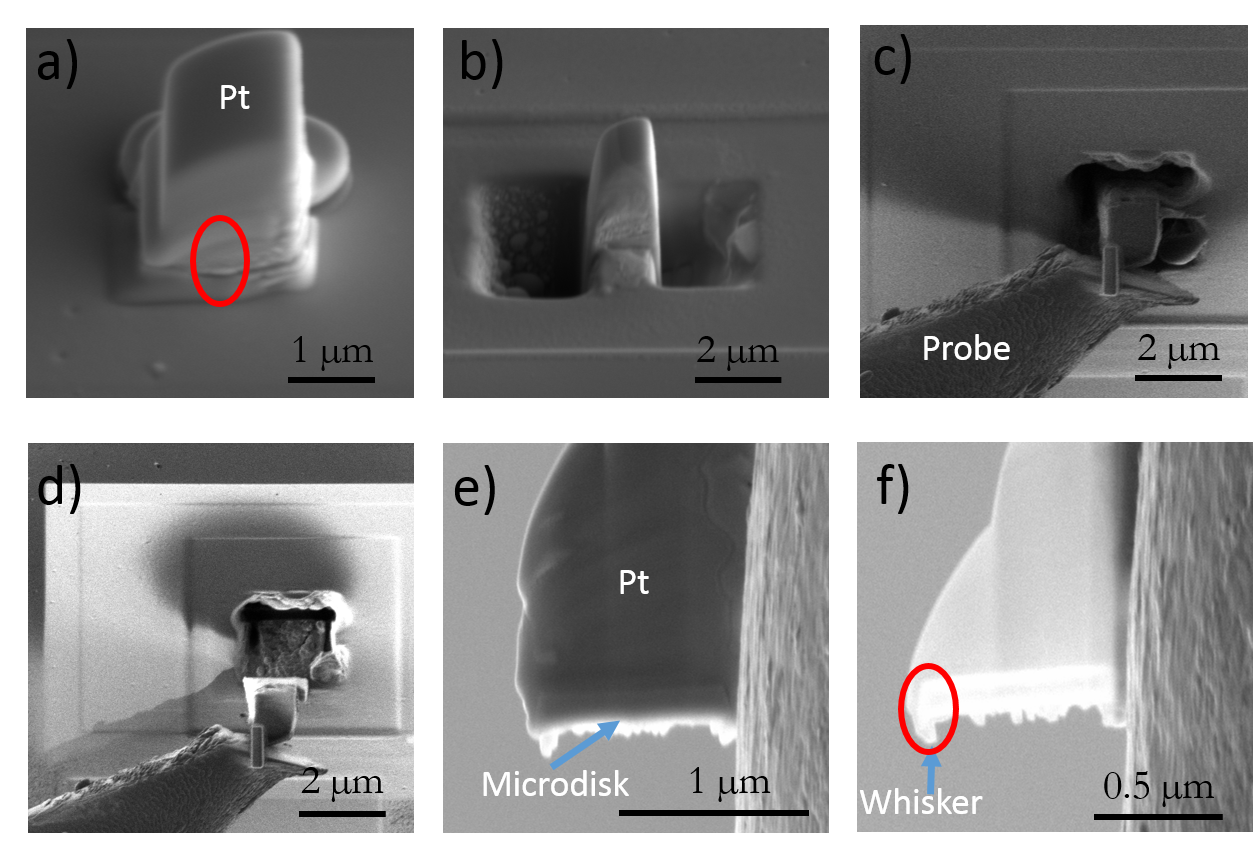
\includegraphics[width=1\textwidth]{Figs/Ch4/udiskliftout}
	\caption {Whisker lift-out process: a) SEM electron beam deposited platinum with the approximate position of the whisker as shown in Fig. \ref{FIBwhisk} circled in red b) milling of trenches by ion beam c)ion-beam image taken after attaching the lift-out probe to the sample using ion-beam deposited Pt and of d) sample release and lift-out e)  SEM image of the initial stages of thinning and f) the final stages of thinning with the whisker visible (red ellipse).}
	\label{udiskliftout}
\end{figure}
\FloatBarrier 

\subsection{STEM}

Following the successful preparation of a TEM lamella, the sample was characterised using STEM-HAADF and BF-STEM. Fig.\ref{whiskerstem}a. shows the presence of a threading dislocation running through the whisker, as well as damage induced by the ion-beam thinning process, illustrating the fragility of the microdisk membrane.

\begin{figure}[h]
	\hspace*{0.5cm}
	\begin{subfigure}[b]{0.48\textwidth}
		\centering
		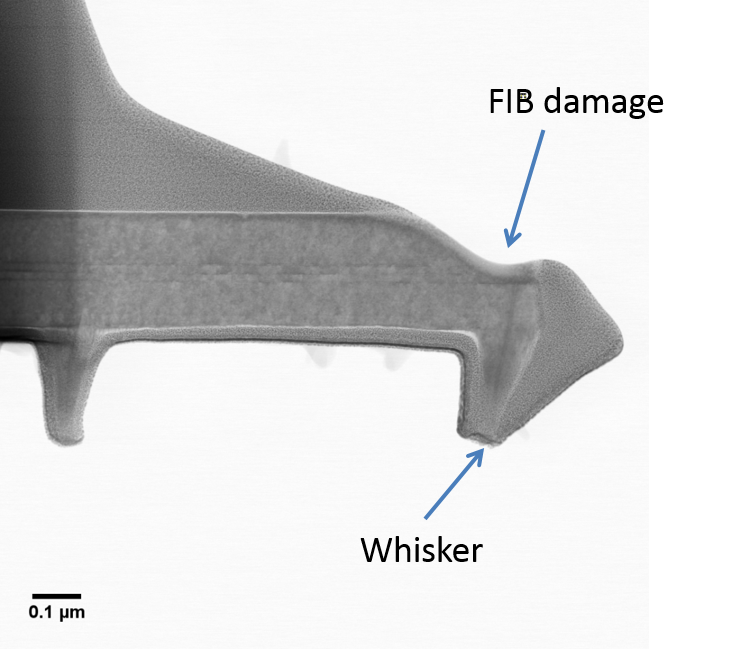
\includegraphics[width=1\linewidth]{Figs/Ch4/whiskBF}
		\caption{}
		
	\end{subfigure}%
	\hspace*{0.5cm}
	\begin{subfigure}[b]{0.48\textwidth}
		\centering
		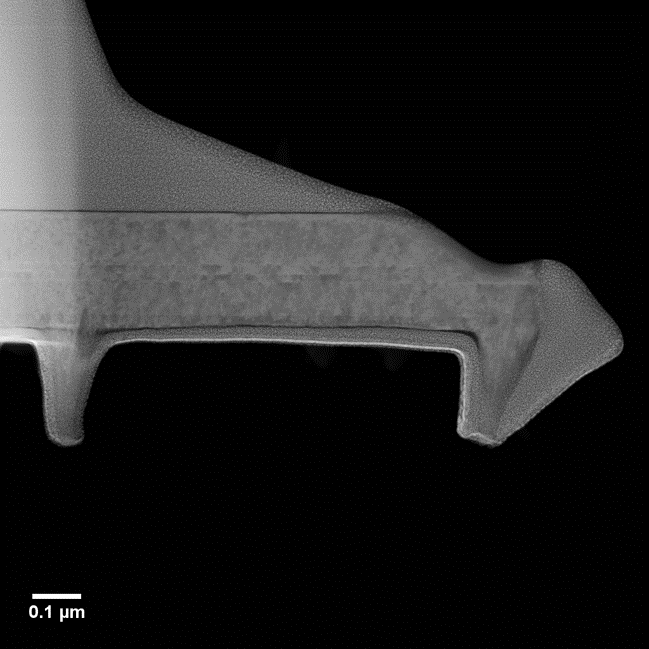
\includegraphics[width=0.86\linewidth]{Figs/Ch4/whiskDF}
		\caption{}
	\end{subfigure}%
	
	\caption{a)BF-STEM and b) STEM-HAADF acquired simultaneously of a TEM lamella prepared containing the microdisk membrane and a whisker. The sample has been slightly damaged by the thinning process.}
	\label{whiskerstem}
\end{figure}
\FloatBarrier

A higher magnification BF-STEM image of the dislocation is shown in Fig.\ref{whiskzoom}, with the dislocation highlighted with a red arrow.

\begin{figure}[h]
	\centering
	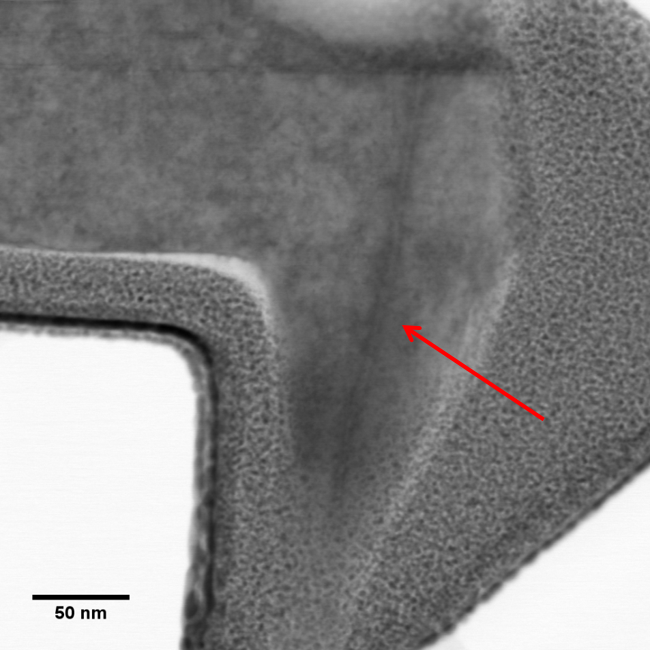
\includegraphics[width=0.4\textwidth]{Figs/Ch4/whiskclosebf}
	\caption {High magnification BF-STEM of the whisker, the red arrow points to the dislocation.}
	\label{whiskzoom}
\end{figure}
\FloatBarrier 

\subsection{WBDF-TEM}

The dislocation was characterised using the WBDF-TEM technique described in section \ref{WBDFsection}. The results are shown in Fig.\ref{whiskerwbdf}. The TD observed here is shown to be a pure edge type dislocation, as shown by the bright constrast produced by the TD when activating \textbf{g} = $<11\bar{2}0>$ (Fig.\ref{whiskerwbdf}.a.) which is absent when activating \textbf{g} = $<0002>$(Fig.\ref{whiskerwbdf}.b.).

\begin{figure}[h]
	
	\begin{subfigure}[b]{0.48\textwidth}
		\centering
		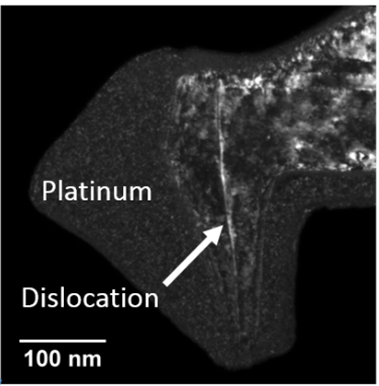
\includegraphics[width=0.92\linewidth]{Figs/Ch4/1120}
		\caption{}
		
	\end{subfigure}%
	\hspace*{0.5cm}
	\begin{subfigure}[b]{0.48\textwidth}
		\centering
		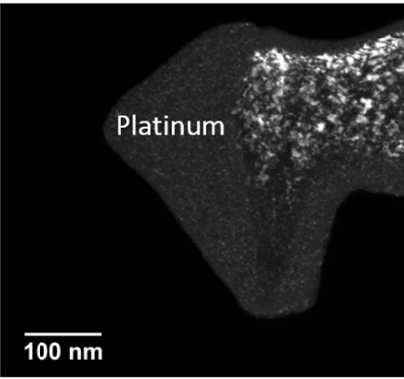
\includegraphics[width=1\linewidth]{Figs/Ch4/0002}
		\caption{}
	\end{subfigure}%
	
	\caption{a)WBDF activating \textbf{g} = $<11\bar{2}0>$  b) WBDF activating \textbf{g} = $<0002>$. The dislocation is only visible along the direction, confirming its nature as a pure edge dislocation.}
	\label{whiskerwbdf}
\end{figure}
\FloatBarrier

These results are the first direct observation of a dislocation within a whisker on the underside of a dislocation. It is expected that mixed, edge and pure dislocations all result in the formation of whiskers under PEC etching \cite{Youtsey1998,Lazar2004}.

\subsection{Active Region Analysis}

The ability to fabricate TEM lamella from microdisks allows unique insight into not only defect-induced whiskers, but also the composition and structure of the active region of the microdisk.

\begin{figure}[h]
	
	\begin{subfigure}[b]{0.48\textwidth}
		\centering
		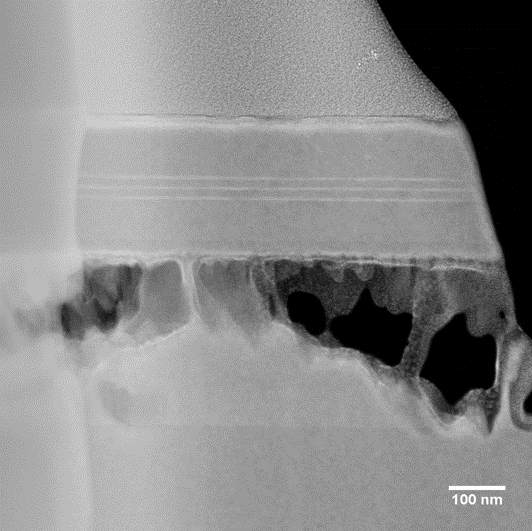
\includegraphics[width=1\linewidth]{Figs/Ch4/microped}
		\caption{}
		
	\end{subfigure}%
	\hspace*{0.5cm}
	\begin{subfigure}[b]{0.48\textwidth}
		\centering
		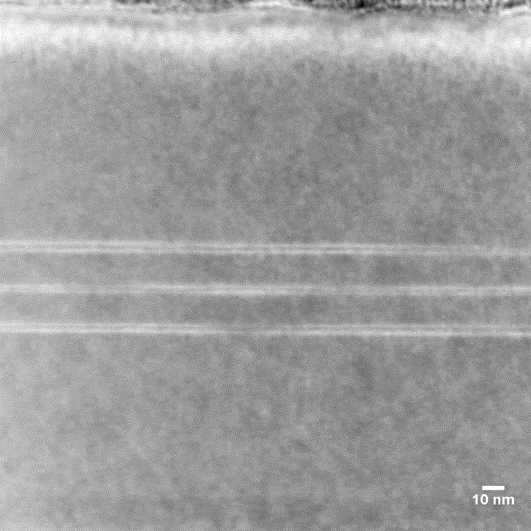
\includegraphics[width=1\linewidth]{Figs/Ch4/micropedzoom}
		\caption{}
	\end{subfigure}%
	
	\caption{a)STEM-HAADF image of a microdisk lamella produced with the membrane, SSL pedestal and \textit{n}-GaN layer and b) higher magnification image of the InGaN active region.}
	\label{pedestal}
\end{figure}
\FloatBarrier
\squeezeup
Fig.\ref{pedestal}.b. shows the apparent 'splitting' of the InGaN QD layers. Compositional mapping was performed to examine the splitting of the layers using EDX and is shown in Fig.\ref{udiskEDX}.\\
Fig.\ref{udiskEDX}.b. shows the In composition reaches close to 0 in between the split lines of the QD containing layer, with a split spacing of approximately 2.5 nm, indicating the layer is close to fully split. As such, the fabrication of TEM lamellae from processed microdisks allows for detailed insight into the structure and composition of the active regions of microdisks providing the potential for correlated measurements between the optical and structural properties of the microdisks.

\begin{figure}
	\begin{subfigure}[b]{0.3\textwidth}
		\centering
		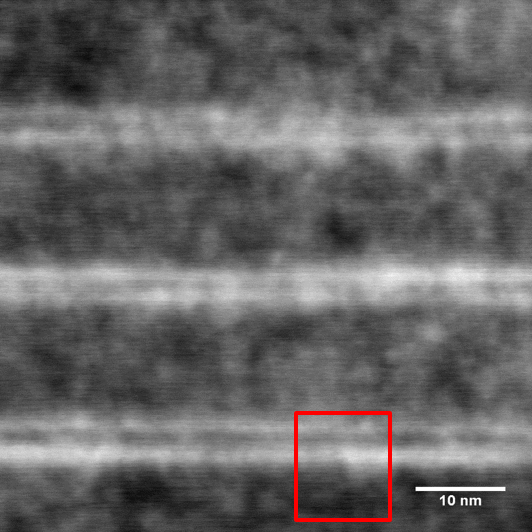
\includegraphics[width=.85\linewidth]{Figs/Ch4/edxtarget}
		\caption{}
		
	\end{subfigure}%
	\hspace*{0.5cm}
	\begin{subfigure}[b]{0.3\textwidth}
		\centering
		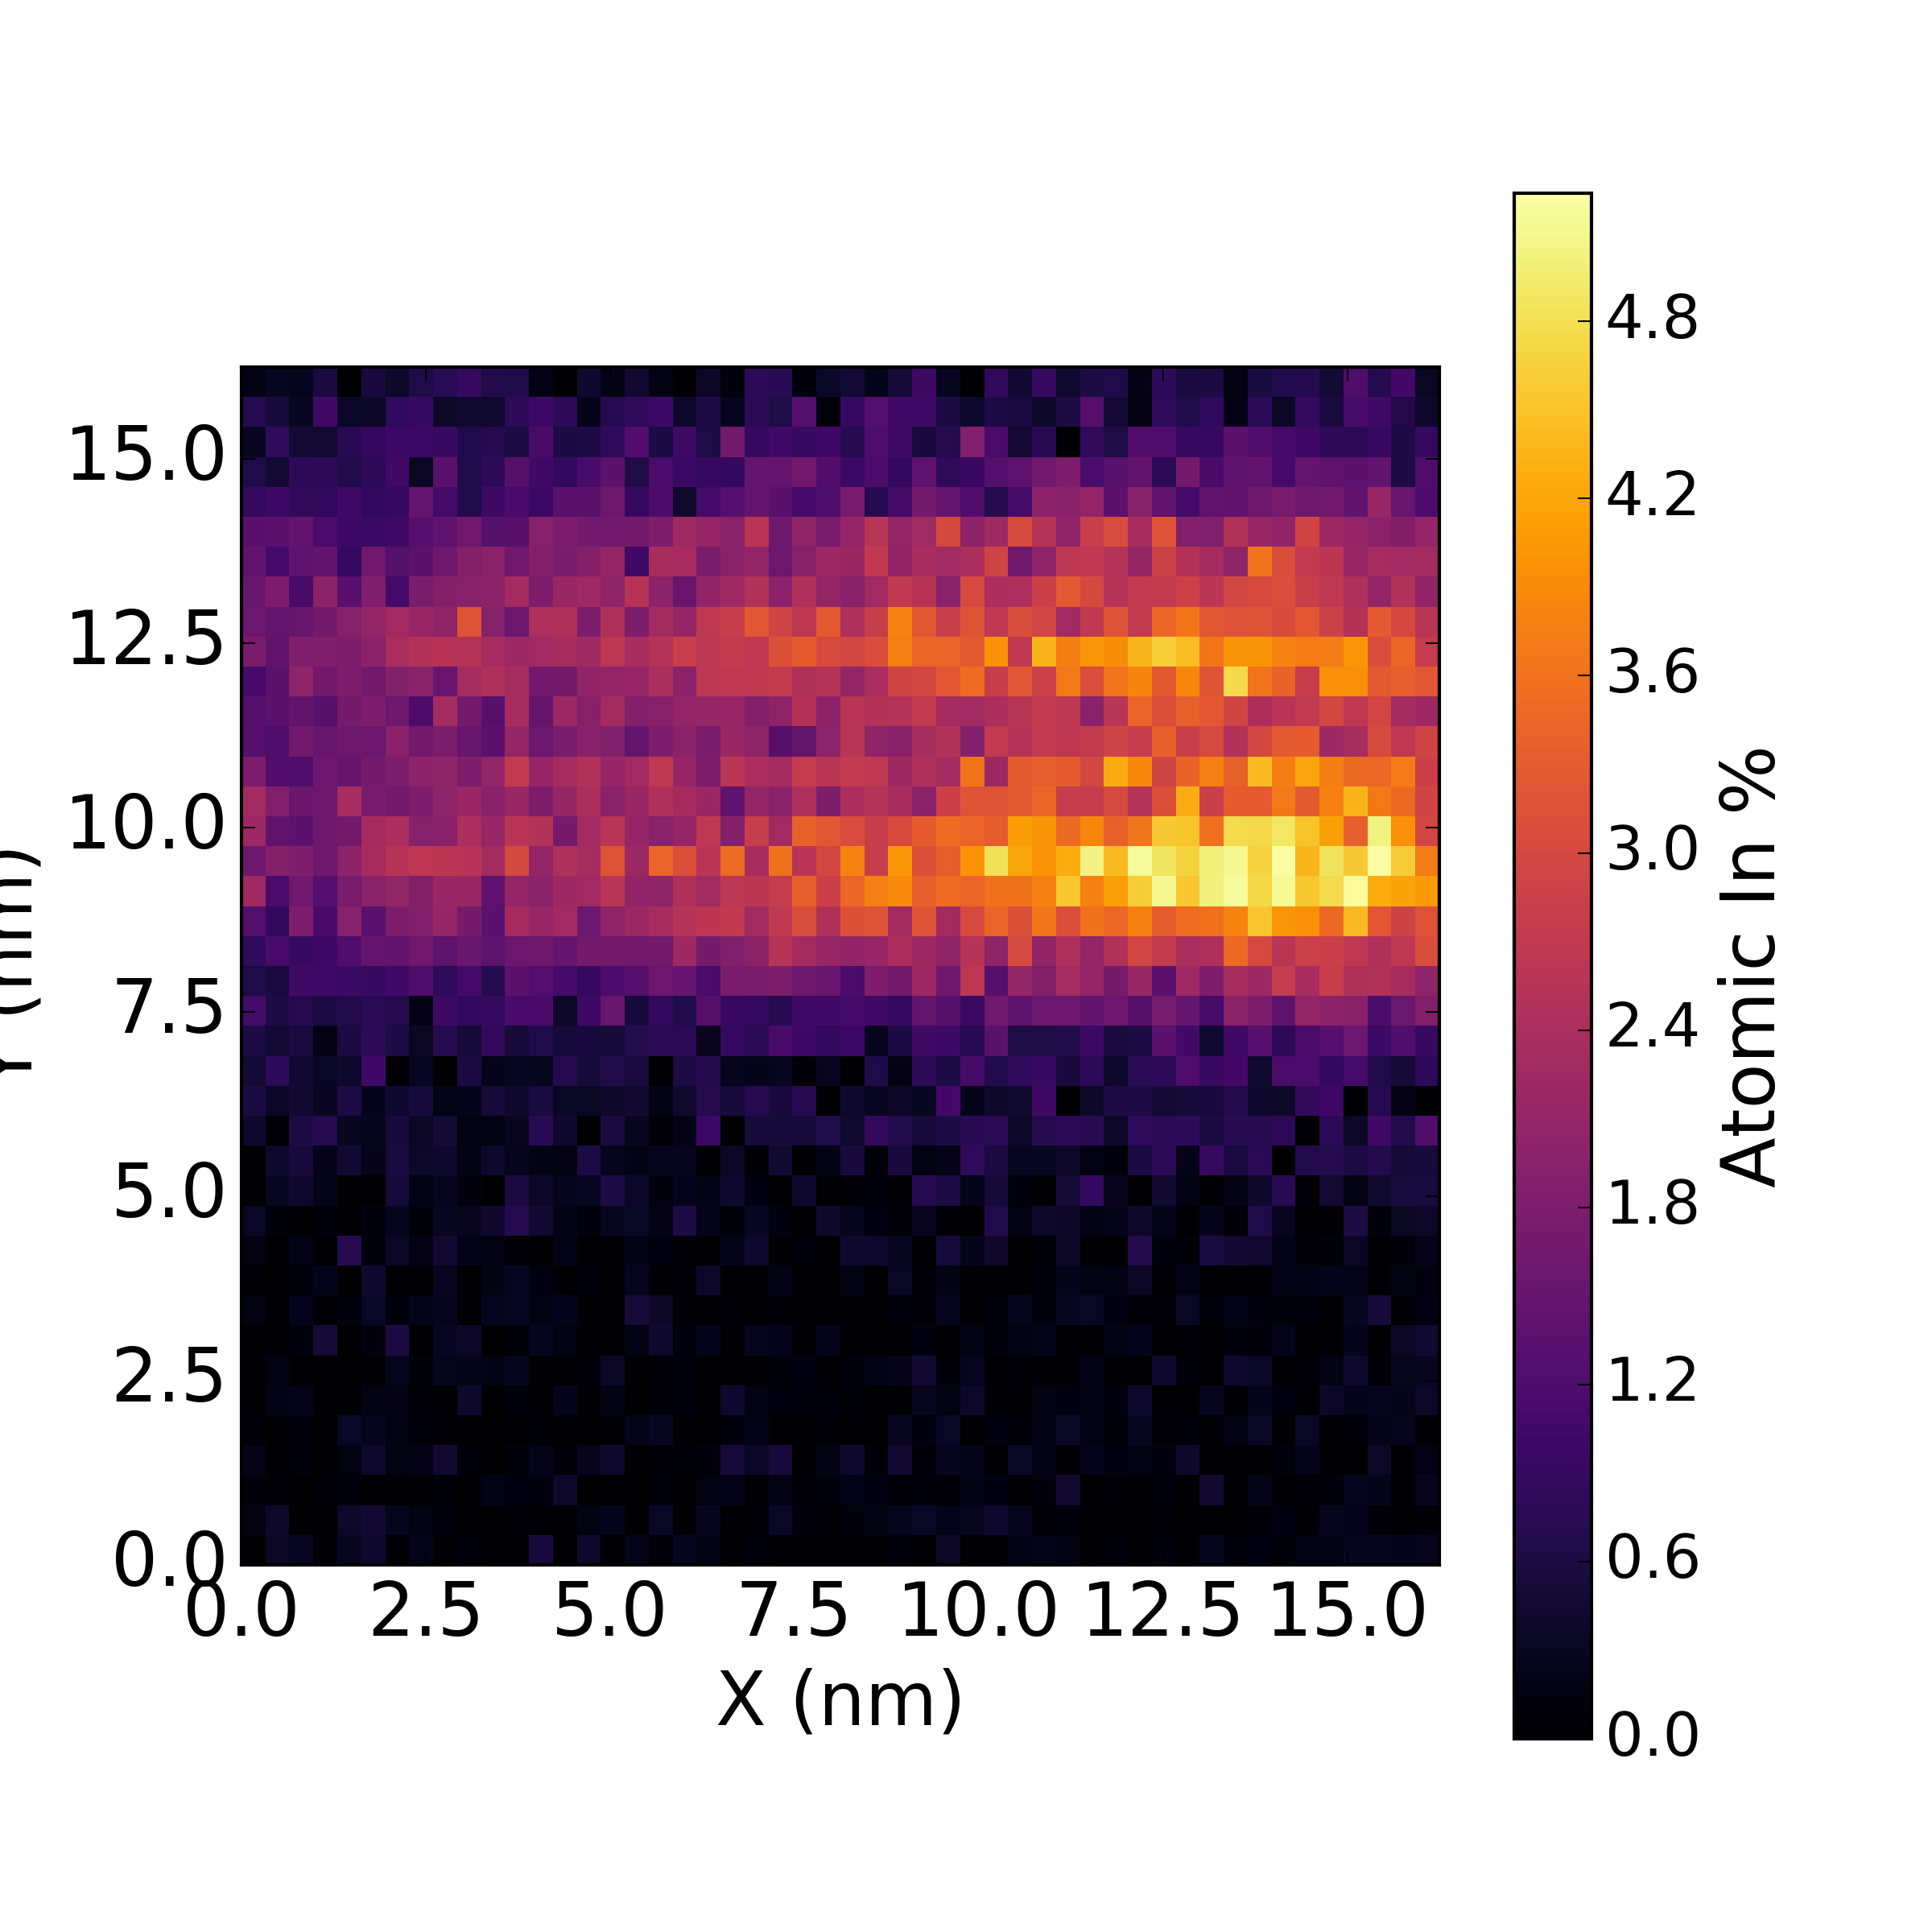
\includegraphics[width=1\linewidth]{Figs/Ch4/AtomicIn}
		\caption{}
		
	\end{subfigure}%
	\hspace*{0.5cm}
	\begin{subfigure}[b]{0.3\textwidth}
		\centering
		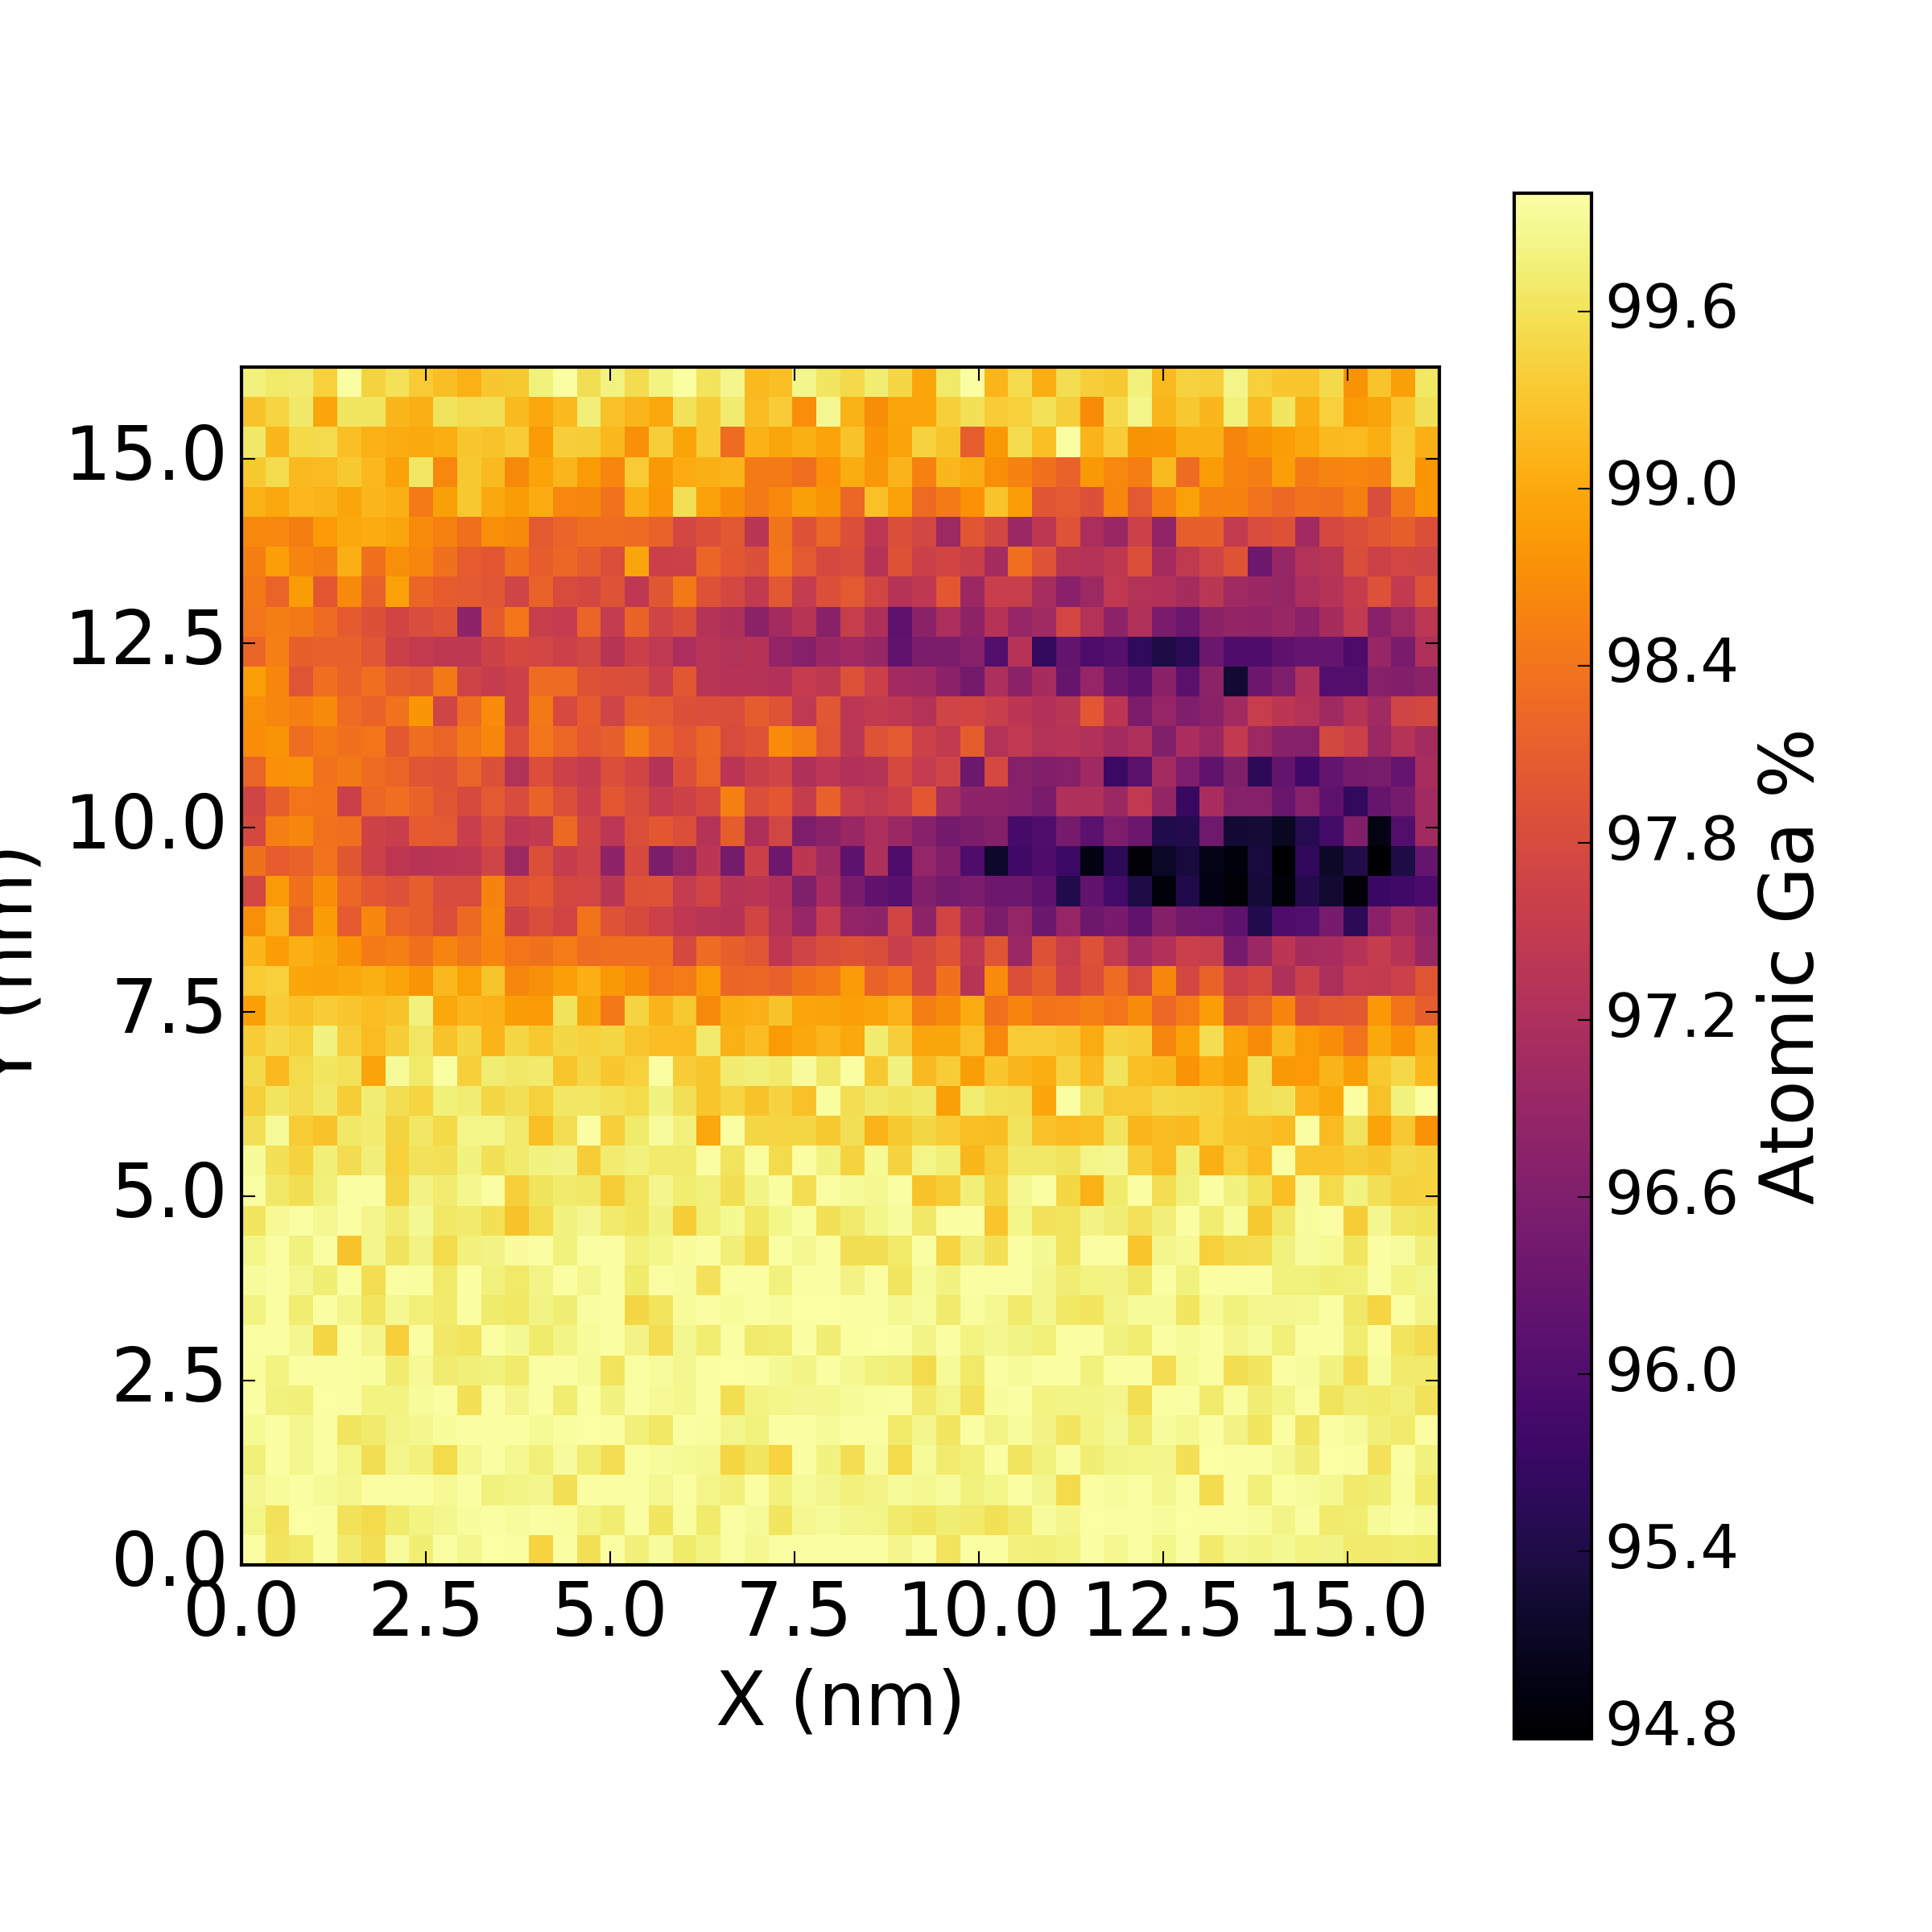
\includegraphics[width=1\linewidth]{Figs/Ch4/AtomicGa}
		\caption{}
	\end{subfigure}%
	
	\caption{a) STEM-HAADF of the active region of the microdisk (scale bar = 10 nm) b) Ga atomic percentage and c) In atomic percentage of the region highlighted in red.}
	\label{udiskEDX}
\end{figure}
\FloatBarrier

\subsection{FIB Tomography}

The mechanism of the PEC etching process causes etching to occur in the presence of photogenerated carriers, as discussed in section \ref{microdisk fab section}. In the case of microdisk membranes containing an InGaN active region the PEC etching process can damage the active region, even with the incorporation of an AlGaN etchstop as discussed in section \ref{microdisk samples}. Beyond potential damage from the PEC etching process, microdisk sidewall and underside roughness can be sources of scattering losses and Q-factor reduction in cavities \cite{Puchtler2015}. FIB tomography provides an easy albeit destructive method of mapping the 3-D morphology of microdisks, potentially providing insight into both issues mentioned above.\\
The microdisks chosen for this tomography study are shown below in Fig.\ref{udisktomotarget}. The damage caused by the PEC etching process to the microdisk membrane is highlighted, as well as the presence of roughness on the underside of the microdisk which is the result of an incomplete PEC etching process.

\begin{figure}[h]
	\centering
	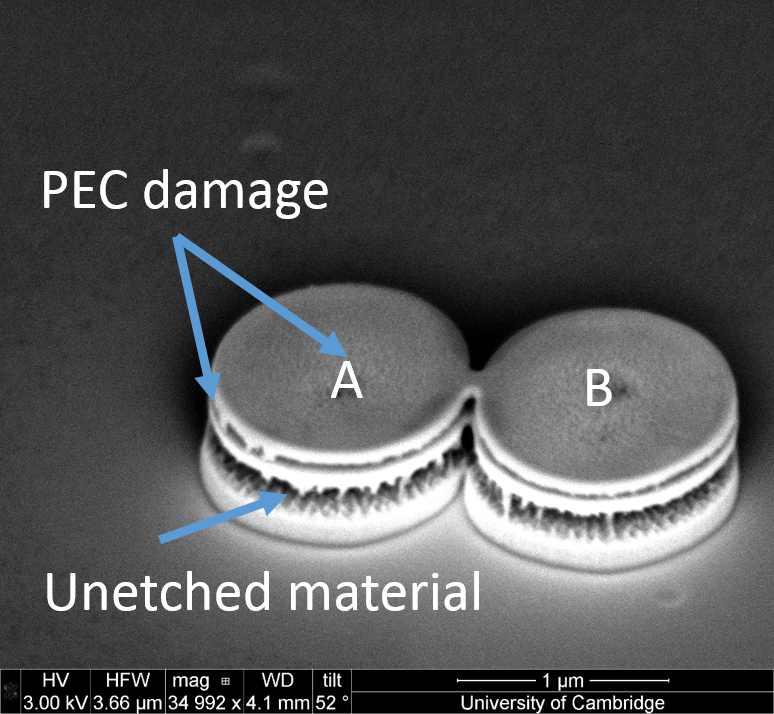
\includegraphics[width=0.4\textwidth]{Figs/Ch4/udisktomo}
	\caption {SEM image of two microdisks exhibiting damage due to the PEC etching process.}
	\label{udisktomotarget}
\end{figure}
\FloatBarrier 
 
As discussed in section \ref{FIBtomo},a protective layer of electron-beam deposited carbon is deposited first on the microdisks as it provides greater contrast with the GaN microdisk in the secondary electron image. Following this, a Pt layer is deposited to provide further protection. An SEM image taken in cross section during the FIB tomography process of the microdisks shown in Fig.\ref{udisktomotarget} is shown in Fig.\ref{slice}.

\begin{figure}[h]
	\centering
	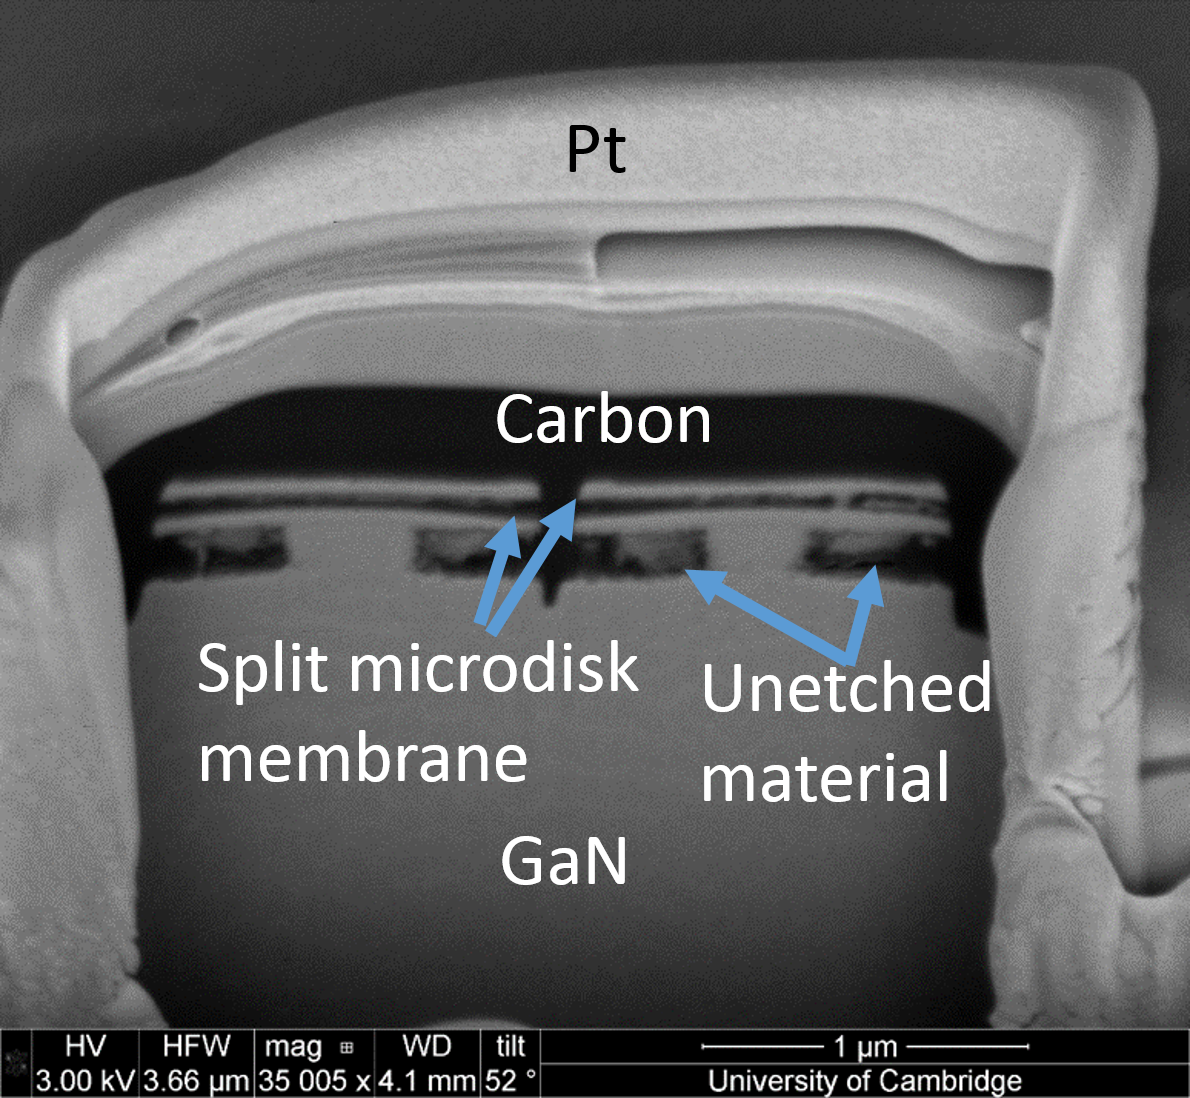
\includegraphics[width=0.5\textwidth]{Figs/Ch4/slice}
	\caption {SEM image of a cross-section of the microdisks shown in Fig.\ref{udisktomotarget}.}
	\label{slice}
\end{figure}
\FloatBarrier 

FIB milling in order to 'slice' the sample was performed at 10 nm step thickness. The reconstruction was performed for the microdisk denoted 'B' in Fig.\ref{udisktomotarget}. Snapshots of the 3D reconstruction are shown in Fig.\ref{tomoreconstruction}. The FEI Helios Nanolab showed poor stability throughout the acquisition, as such a complete series containing the microdisk could not be acquired. The datasets were aligned using Avizo 7, which includes stretching in order to compensate for the acquisition angle for the SEM images.

\begin{figure}
	\begin{subfigure}[b]{0.45\textwidth}
		\centering
		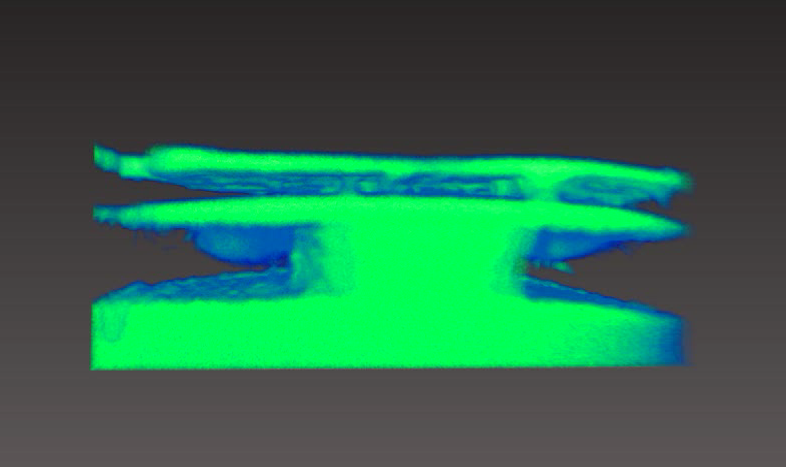
\includegraphics[width=1\linewidth]{Figs/Ch4/tom1}
		\caption{}
	\end{subfigure}%
	\hspace*\fill
	\begin{subfigure}[b]{0.45\textwidth}
		\centering
		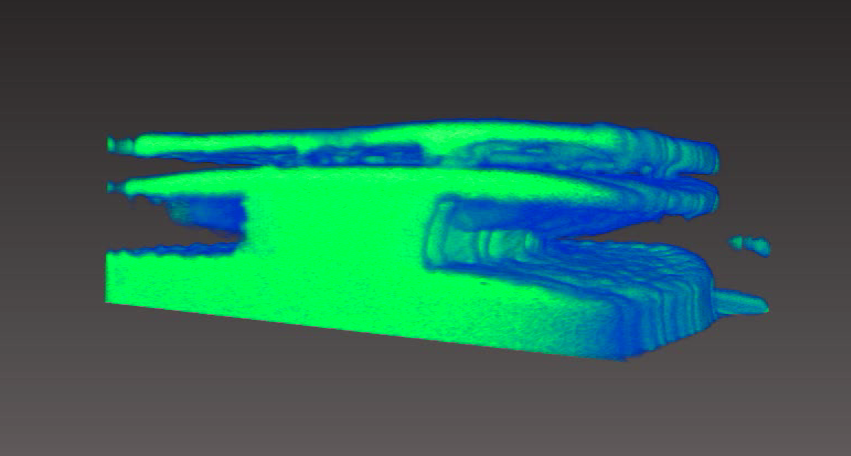
\includegraphics[width=0.98\linewidth]{Figs/Ch4/tom2}
		\caption{}		
	\end{subfigure}%
	
	\medskip
	\begin{subfigure}[b]{0.45\textwidth}
		\centering
		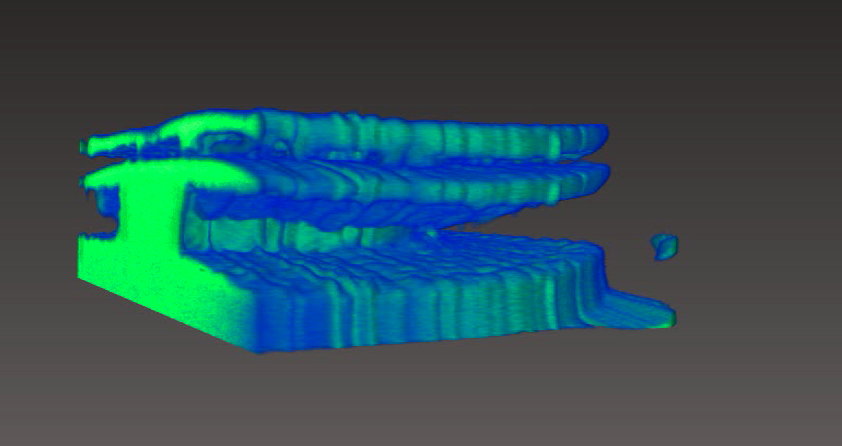
\includegraphics[width=1\linewidth]{Figs/Ch4/tom3}
		\caption{}
	\end{subfigure}%
	\hspace*\fill
	\begin{subfigure}[b]{0.45\textwidth}
		\centering
		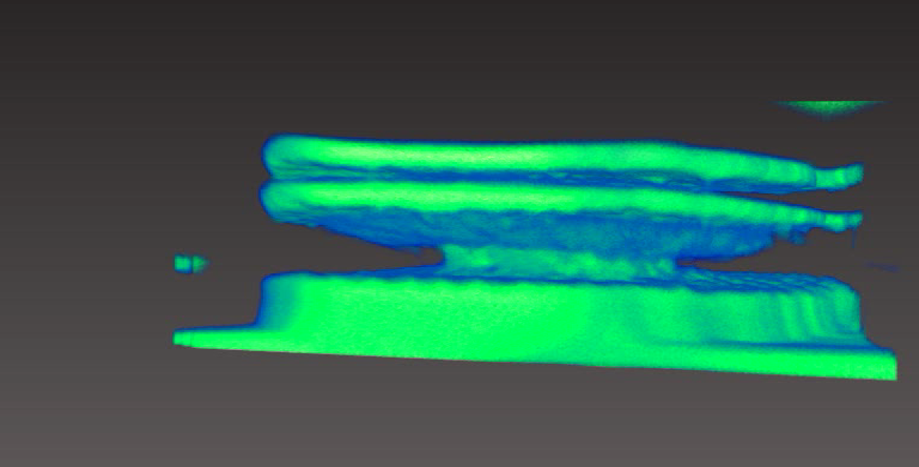
\includegraphics[width=1\linewidth]{Figs/Ch4/tom5}
		\caption{}		
	\end{subfigure}%
	
	\medskip
	\begin{subfigure}[b]{0.45\textwidth}
		\centering
		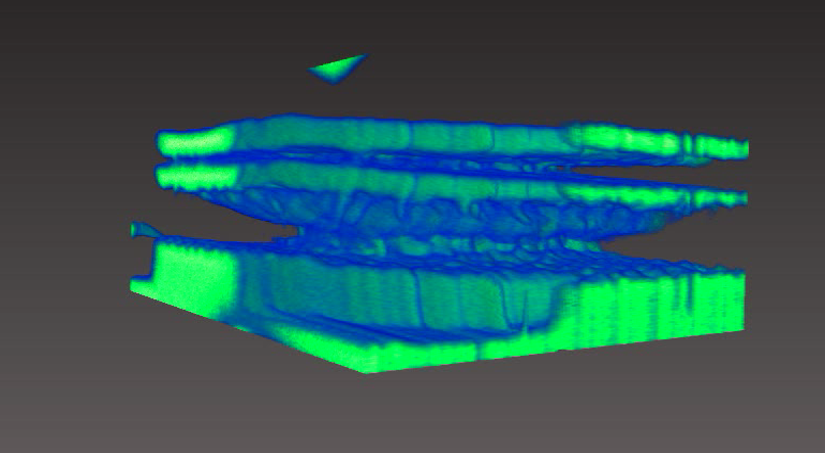
\includegraphics[width=1\linewidth]{Figs/Ch4/tom6}
		\caption{}
	\end{subfigure}%
	\hspace*\fill
	\begin{subfigure}[b]{0.45\textwidth}
		\centering
		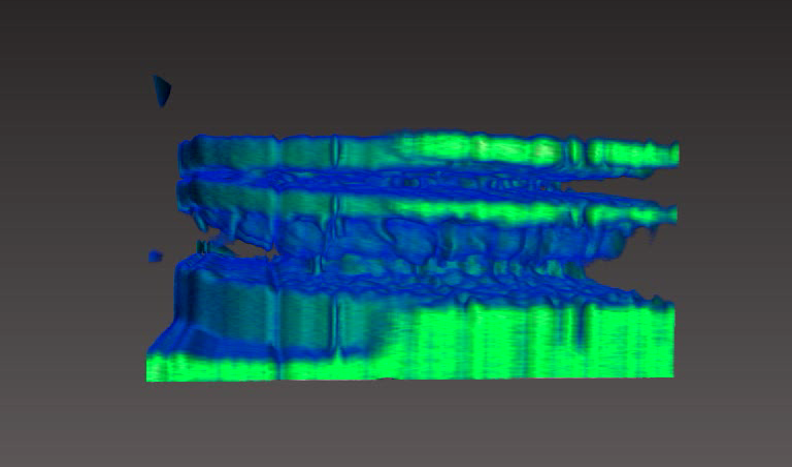
\includegraphics[width=1\linewidth]{Figs/Ch4/tom7}
		\caption{}		
	\end{subfigure}%
	
	\caption{Tomographic reconstruction for microdisk 'B'.}
	\label{tomoreconstruction}
\end{figure}

\FloatBarrier 

\subsubsection{Analysis}

In order to perform quantitative analysis of the microdisk, the image stack generated through the tomography experiment was reconstructed into an isosurface through the use of a marching cubes algorithm \cite{Lorensen1987} implemented in the scikit-image python package. The algorithm generates a surface from a triangular mesh, thus allowing us to access information concerning the surface of the microdisk down to the resolution of the SEM images in x-y plane, and the slice thickness in the z-direction. In this set of images the pixel size in each image is 1.2 nm, and the slice thickness is 10 nm.\\
Reconstruction using scikit-image allows us to access specific parts of the microdisk. In this instance we are interested in the top portion of the 'split' microdisk membrane. Fig.\ref{mayavi1} shows a reconstruction of this region.

\begin{figure}[h]
	\centering
	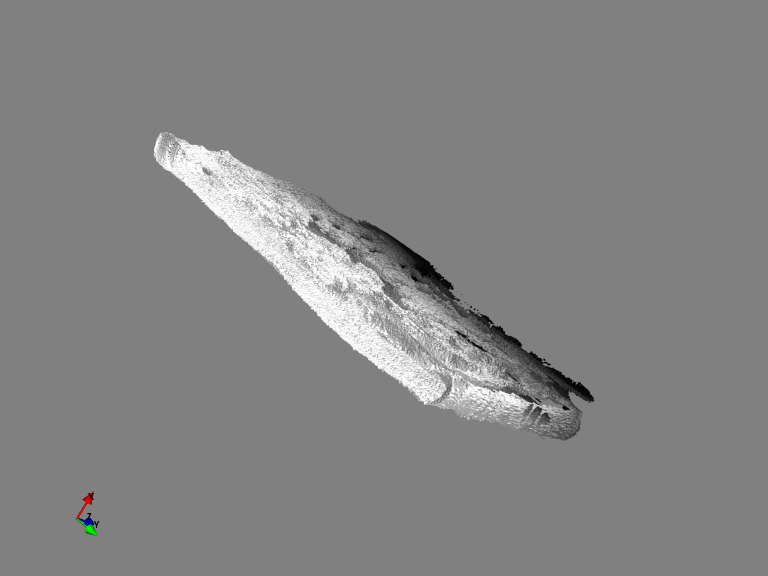
\includegraphics[width=0.5\textwidth]{Figs/Ch4/membrane.png}
	\caption {Isosurface reconstruction of the top portion of the microdisk membrane}
	\label{mayavi1}
\end{figure}
\FloatBarrier 

Fig.\ref{mayavi2} shows a top view of the reconstructed membrane, demonstrating the sub-optimal stacking of the image slices as the perimeter of the microdisk membrane seems distorted from it's expected circular shape. A certain amount of 'roughness' in the microdisk can be seen on the surface.

\begin{figure}[h]
	\centering
	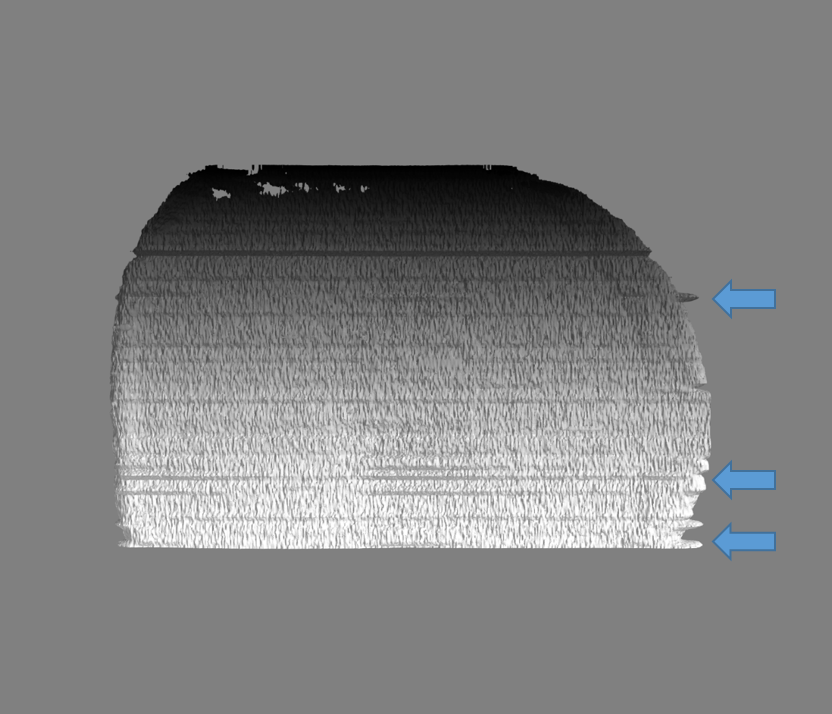
\includegraphics[width=0.5\textwidth]{Figs/Ch4/udisktomoarrowstop.png}
	\caption {Top view of the reconstructed isosurface. Blatant stacking errors are denoted by blue arrows.}
	\label{mayavi2}
\end{figure}
\FloatBarrier

In order to quantify this roughness, we utilise a method described by Vartak \textit{et al.} \cite{Vartak2016}. The triangular mesh generated by the marching cubes algorithm is composed of triangles represented by vertices. As such, the cross product of any two of vectors between two vertices gives the normal vector of the triangle such that:

\begin{equation}
\textbf{A} \times \textbf{B} = |A||B|sin(\theta)\textbf{N}
\end{equation}

where $\theta$ is the angle between the two vectors \textbf{A} and \textbf{B}
This is shown schematically in Fig.\ref{crossprod}.

\begin{figure}[h]
	\centering
	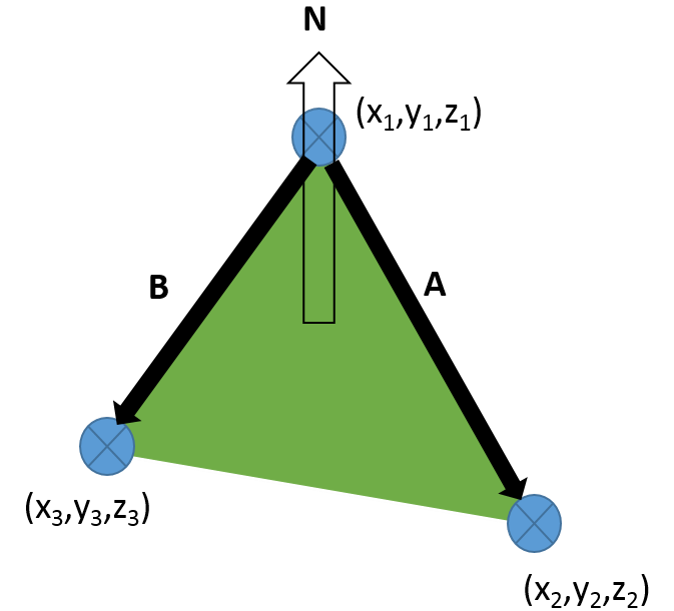
\includegraphics[width=0.4\textwidth]{Figs/Ch4/crossprod.png}
	\caption {The cross product of any two vectors (\textbf{A} and \textbf{B}) describing two facets of a triangle in the triangular mesh gives the area normal vector \textbf{N}.}
	\label{crossprod}
\end{figure}
\FloatBarrier

The dot product of the normal vectors for each triangle and a vector representing an ideal flat surface gives the angle of orientation of each individual triangle composing the isosurface. The angle between the ideal surface vector \textbf{F} and any triangle with an area vector \textbf{N} in the mesh is then given by the relation:

\begin{equation}
\phi = arcos((\textbf{F}\cdot\textbf{N})(|\textbf{F}||\textbf{N}|))
\end{equation}

As shown schematically in Fig.\ref{dotprod}. 

\begin{figure}[h]
	\centering
	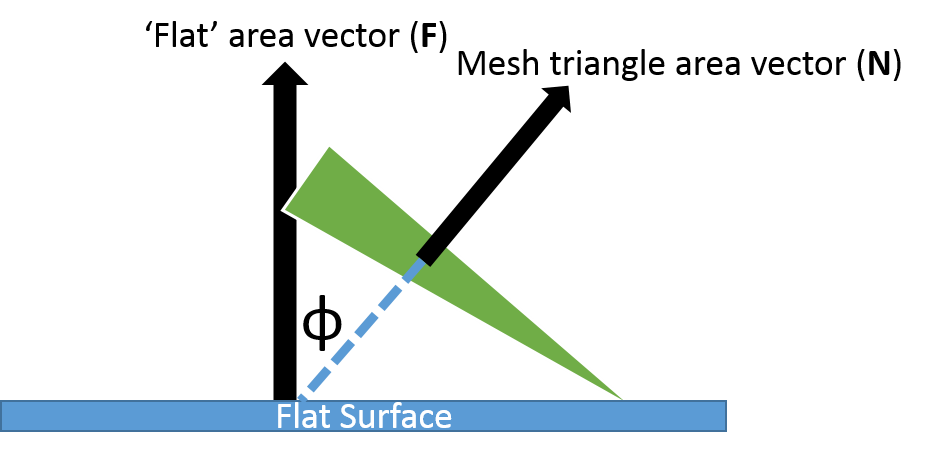
\includegraphics[width=0.4\textwidth]{Figs/Ch4/roughnessangle.png}
	\caption {The dot product between the normal vector of a triangle in the mesh and an ideal flat surface gives the angle}
	\label{dotprod}
\end{figure}
\FloatBarrier


As such, the variance of these angles correspond to variations in the orientation of the triangles composing the isosurface and can be interpreted as a measure of corrugation, or roughness. This is highly dependent on the orientation of the surface, the side walls of the isosurface will require a different 'ideal' flat surface relative to the top surface of the microdisk membrane. This method yields an angular variance of $1.5 \times 10^{-3}$ degrees for the surface shown in Fig.\ref{mayavi1}.\\
Performing smoothing and noise removal on the individual SEM images comprising the stack should allow for a smoother surface reconstruction as shown in Fig.\ref{smoothmayavi}. 

\begin{figure}[h]
	\hspace*{0.5cm}
	\begin{subfigure}[b]{0.48\textwidth}
		\centering
		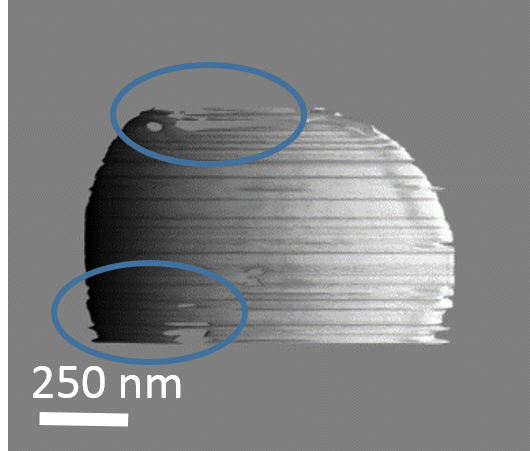
\includegraphics[width=1\linewidth]{Figs/Ch4/may2}
		\caption{}
		
	\end{subfigure}%
	\hspace*{0.5cm}
	\begin{subfigure}[b]{0.48\textwidth}
		\centering
		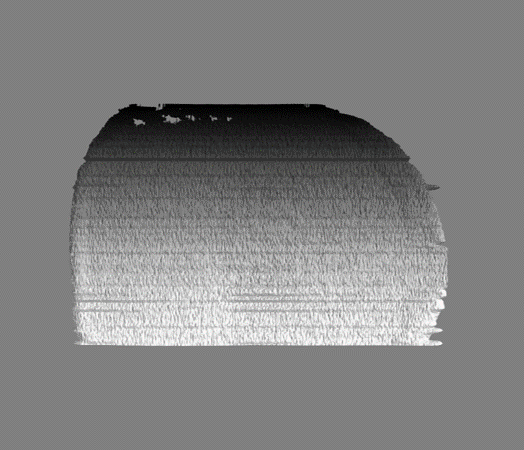
\includegraphics[width=1\linewidth]{Figs/Ch4/may1}
		\caption{}
	\end{subfigure}%
	
	\caption{a) Smoothed isosurface b) unsmoothed.}
	\label{smoothmayavi}
\end{figure}
\FloatBarrier
 
The smoothed surface yields an angular variance of $8.3 \times 10^{-4}$ degrees, indicating the angular variance can indeed be used as a measure of roughness in analysing the reconstruction. However, the thresholding in the smoothing process can be seen to result in the generation of some 'holes' in the membrane, which may introduce artificial roughness into the calculation.

\section{Summary}
The PEC etching process provides an effective manner in undercutting GaN microdisk membranes. However, due to the mechanism of etching which relies on the presence of photo-generated carriers, dislocations can hinder the etching process resulting in the formation of 'whiskers' of unetched material on the underside of the microdisk, which provide a radiative pathway for WGMs propagating in the microdisk to escape thus reducing cavity Q-factor.\\
In this chapter, we have presented a manner through which TEM lamellae can be prepared from processed microdisks. Following this we have performed TEM in order to reveal the presence of a dislocation at the centre of a whisker. Using WBDF-TEM we have identified the dislocation type as pure edge, though mixed and pure screw dislocations are expected to result in the formation of whiskers. This preparation method has also allowed us to examine the active region in the microdisk membrane using STEM-HAADF and STEM-EDX, revealing the presence of a 'split' InGaN active region.\\
Fig.\ref{tomoreconstruction}. demonstrates the ability of the FIB tomography process to access detailed information concerning the morphology of the disk. The 'splitting' of the microdisk membrane caused by etching of the active region can be seen in reconstruction, as well as residual material on the underside of the microdisk indicating incomplete etching. FIB tomography thus provides a reliable albeit destructive manner of accessing microdisk morphology, which could potentially be utilised in conjunction with optical characterisation techniques for correlated measurements.

\section{Future Work}
A continuation of the work presented in this chapter would likely involve correlated optical and structural measurements. In particular, the TEM lamella preparation allows for insight into the active region of microdisks. As such, an experiment involving the correlation between PL, CL and site-specific STEM-EDX would allow for a comprehensive analysis of the optical and structural properties of the InGaN active region, as well as its interaction with the microdisk cavity. Beyond this, the groundwork for the analysis of the 3D morphology of the microdisks has been presented here, in extending this with AFM measurements of the microdisk membrane surface the accuracy and precision of the tomographic reconstruction may be reassessed. Following this, roughness measurements obtained via FIB tomography coupled with cavity Q-factor measured through micro-PL may provide insight into current fabrication limitations.







